\chapter{مقدمه}
\section{مقدمه}

استفاده روز افزون از سامانه‌های تشخیص هوشمند چهره موجب اهمیت این شاخه از علم هوش مصنوعی شده است. هدف این است که تصویری به کامپیوتر داده شود و سامانه تشخیص دهد که آیا چهره‌ای در تصویر مشاهده می‌کند یا خیر، و در صورت وجود چهره، در صورت امکان آن را شناسایی نماید. عملکرد این سامانه‌ها در شرایط کنترل شده و آزمایشگاهی به حد مناسبی از بلوغ رسیده است. اما تشخیص چهره در شرایط کنترل نشده، موضوعی چالش برانگیز و در حال پیشرفت می‌باشد. در شرایط مختلفی مانند تابش نور غیر یکنواخت، زاویه نامناسب چهره در مقابل دوربین، وضوح پایین حسگر و... گاهی چهره‌ای یافت نمی‌شود و یا چهره یافت شده، قابل شناسایی نمی‌باشد. این مشكلات در سامانه‌های تشخیص چهره مبتنی بر ویدیو، به دلیل عدم ثبات شرایط محیطی و انسانی، تاثیر بیشتری داشته و در نتیجه، باعث کاهش دقت سامانه در تشخیص افراد می‌شود.

\noindent
در این بخش به منظور آشنایی کلی با موضوع مورد پژوهش، ابتدا توضیح مختصری در مورد ویژگی‌های بیومتریک انسان و ارزیابی آن‌ها آورده شده است. پس از آن به طور خاص بر روی ویژگی بیومتریک چهره متمرکز شده و در مورد کاربردها، انواع، مراحل، بخش‌ها، مزایا و چالش‌های آن به طور کامل بحث شده است. سپس به تعریف یک مسئله خاص در زمینه تشخیص چهره به صورت بی‌درنگ و در محیط کنترل نشده پرداخته و نیاز‌ها و ابزارهای مورد نیاز بررسی شده است.

\section{ویژگی‌های بیومتریک}
امروزه در زمینه‌های فراوانی نیاز به سامانه‌ای می‌باشد که هویت اشخاص را بر اساس ویژگی‌های بدن آن‌ها شناسایی کند. این زمینه علمی علاقه مندان فراوانی پیدا کرده و استفاده از ویژگی‌های بیومتریک \LTRfootnote{Biometric} در سال‌های اخیر به صورت گسترده مورد استفاده قرار گرفته است. این ویژگی‌ها در هر شخص منحصر به فرد است که از آن جمله می‌توان به اثر انگشت، گفتار، نوع راه رفتن و چهره اشاره کرد. ویژگی های بیومتریک را نمی‌توان امانت داد یا قرض گرفت. نمی‌توان خرید یا فراموش کرد و جعل آن هم تقریبا غیر ممکن است. یک سامانه بیومتریک در واقع یک سامانه تشخیص الگو است که یک شخص را بر اساس ویژگی‌های خاص فیزیولوژیک بازشناسی می‌کند. 

\subsection{ارزیابی ویژگی‌های بیومتریک انسان}

معمولا ویژگی‌های بیومتریک انسان با 8 عامل مورد ارزیابی قرار می‌گیرند \cite{Biometrics} که عبارت اند از:
\begin{enumerate}
\item
 عمومیت: هر شخصی باید دارای آن ویژگی بیومتریک باشد.
 \item
 یکتایی: آن ویژگی بیومتریک باید برای هر شخصی منحصر بفرد باشد.
 \item
 دوام: معیاری برای سنجش آنکه یک ویژگی بیومتریک چه مدت بدون تغییر باقی می‌ماند.
 \item
 ارزیابی: ویژگی بیومتریک مورد نظر باید سادگی کافی را در استفاده برای ارزیابی نمونه‌های متفاوت داشته باشد.
 \item
 کارایی: استفاده از ویژگی بیومتریک مورد نظر باید دقت، سرعت و پایداری مطلوب داشته باشد.
 \item
 مقبولیت: فناوری استفاده از ویژگی بیومتریک مورد نظر باید در میان جامعه پذیرش شده باشد.
 \item
 تصدیق هویت: ویژگی فرد به سامانه ارسال شود و سامانه پاسخی مثبت یا منفی برای تصدیق هویت فرد ارائه نماید.
 \item
 تشخیص هویت: ویژگی فرد به سامانه ارسال ‌شود و سامانه با جستجو در پایگاه داده، هویت فرد را استخراج نماید.
\end{enumerate} 

\noindent
ویژگی بیومتریک چهره تمام موارد بالا را شامل می‌شود و یکی از بهترین انتخاب‌ها برای طراحی یک سامانه تشخیص هویت می‌باشد. پس از موفقیت سامانه شناسایی از طریق اثر انگشت در چند سال اخیر، فناوری تشخیص چهره یکی از مهم‌ترین فناوری‌های بیومتریک برای شناسایی افراد محسوب می‌شود.

\section{سامانه تشخیص چهره}

تشخیص چهره همواره یکی از موضوعات مورد مطالعه در علوم کامپیوتر و هوش مصنوعی بوده است.  این اهمیت و توسعه کاربرد به دو دلیل مهم می‌باشد:

\begin{enumerate}
\item
	تشخیص چهره برای استفاده در کاربردهای مختلف مانند کاربرد‌های امنیتی، قابلیت شناسایی خودکار سریع و بدون دخالت شخص را دارد، سرعت پردازش را بالا برده و خطا را کاهش داده است.
\item 
سامانه تشخیص چهره نسبت به سامانه‌های بیومتریک قابل اعتمادی مانند تشخیص اثر انگشت و عنبیه چشم، ارتباط راحت‌تری با کاربر ایجاد کرده و بدون تماس عضوی از بدن با سامانه، عملیات تشخیص انجام می‌گیرد. البته توسعه کاربردهای دوربین‌های دیجیتالی پیشرفته عامل موثری در توسعه و بالا رفتن طرفداران این سامانه بوده است.
\end{enumerate}

سامانه تشخیص چهره بر اساس الگوریتم‌های شناسایی و مقایسه تصاویر کار می‌کند. اساس و پایه این الگوریتم‌ها شناسایی و تجزیه و تحلیل ویژگی‌های مربوط به اندازه، شکل و موقعیت چشم، بینی، گونه‌ها و اعضای چهره می‌باشد. تصاویر رقمی برای سامانه ارسال می‌شود و سامانه به طور خودکار چهره شخص را در تصویر پیدا می‌نماید و ویژگی‌های آن را استخراج و با نمونه‌های دیگر مقایسه می‌کند. نتیجه این پردازش، لیستی از هویت‌ها است که رتبه بندی شده است.

\subsection{کاربردها و ویژگی‌های مهم سامانه تشخیص چهره}

فناوری تشخیص چهره که دارای مزایایی چون دقت بالا و سطح پایین دخالت فرد می‌باشد، در مواردی مانند کنترل دسترسی \LTRfootnote{Access Control}، امنیت اطلاعات، اجرا و نظارت بر قانون، شناسایی مجرمین، کنترل و ثبت تردد در سامانه‌های حضور و غیاب، کنترل نامحسوس و ایجاد امنیت در بانک، فروشگاه، فرودگاه و... مورد استفاده قرار می‌گیرد و در صنعت و علم مورد توجه قرار گرفته است.

\noindent
علاوه بر کاربردهای فوق، شناسایی و پردازش چهره کاربردهای دیگری هم دارند که ارتباطی با تشخیص هویت ندارند. دنبال کردن خط دید چشم و تعیین نژاد، جنس، سن و حالت صورت از جمله این کاربردها هستند که بعضی از آن‌ها در ارتباط بین انسان و کامپیوتر مفید هستند. کاربردهای زیادی برای مباحث شناسایی چهره می‌توان متصور شد که محدوده وسیعی از تصاویر متحرک تا تصاویر ثابت و از کاربردهای امنیتی تا کاربردهای تجاری را شامل می‌شود. این کاربردها را بر اساس نوع تصاویری که استفاده می‌کنند، می‌توان به دو گروه تصاویر ثابت و متحرک تقسیم کرد که در مواردی همچون کیفیت تصویر، زمینه تصویر، در دسترس بودن معیار انطباق و... با یکدیگر تفاوت دارند. دو ویژگی مهم یک سامانه تشخیص چهره عبارتند از:

\noindent
سرعت تشخیص: بدین معنا که یک الگوریتم تشخیص چهره از لحظه قرارگیری فرد در مقابل دوربین، در چه بازه زمانی می‌تواند هویت فرد درون تصویر را تشخیص دهد.

\noindent
دقت تشخیص: بدین معنا که یک الگوریتم تشخیص چهره با چه ضریب اطمینانی می‌تواند هویت یک فرد درون تصویر را تشخیص دهد. هرچه تعداد افراد مختلفی که در پایگاه داده ثبت نام شده اند، بیشتر باشد، احتمال خطا در سامانه بیشتر می‌شود و به یک الگوریتم دقیق تر نیاز داریم.

\noindent
بین سرعت تشخیص و دقت تشخیص، بده بستان \LTRfootnote{Tradeoff} وجود دارد. یک الگوریتم کارا باید هر دو ویژگی بالا را در نظر بگیرد.

\subsection{نمای کلی یک سامانه تشخیص چهره}

یک سامانه بیومتریک تشخیص چهره شامل بخش‌های مختلفی می‌باشد که در شکل \ref{image1-1} نشان داده شده است. شش بخش مهم یک سامانه تشخیص چهره عبارتند از:

\noindent
حسگر دوربین: این بخش وظیفه گرفتن تصویر چهره را بر عهده دارد. دستگاه گیرنده بسته به نیاز و کاربرد می‌تواند یک دوربین سیاه و سفید، رنگی، یک دوربین مخصوص با قابلیت استخراج اطلاعات عمق یا یک دوربین مادون قرمز باشد.

\noindent
یافتن چهره: تصاویر ورودی به این بخش ابتدا مورد پیش پردازش قرار می‌گیرند. سپس ارزیابی محتوایی شده و داده‌های نامربوط از قبیل پس زمینه، موها و گردن و شانه و... حذف می‌شوند و تنها ناحیه چهره باقی می‌ماند.

\noindent
تراز کردن چهره: چهره پیدا شده در مرحله قبل، تراز می‌شود. به گونه ای که چشم ها در راستای افقی قرار بگیرند.

\noindent
استخراج اطلاعات: در این بخش ویژگی‌های چهره مورد بررسی قرار گرفته و اطلاعات مورد نیاز از تصویر استخراج می‌گردد تا با تصاویر موجود در پایگاه داده مقایسه گردد.

\noindent
پایگاه داده: این بخش وظیفه ثبت نام، نگهداری و واکشی ویژگی چهره کاربران را بر عهده دارد. پایگاه داده مجموعه‌ای از تصاویر است که در مرحله طبقه‌بندی مورد استفاده قرار می‌گیرد. در بیشتر روش‌های تشخیص چهره چندین نمای متفاوت از یک شخص در حالت‌های مختلف روحی خنده، اخم، عصبانیت، عادی و یا با عینک از کاربر گرفته می‌شود که موجب بالا رفتن ضریب شناسایی سامانه می‌شود.

\noindent
طبقه‌بندی: در این بخش ویژگی‌های استخراج شده با ویژگی‌های موجود در پایگاه داده تصاویر مقایسه می‌گردد و مشخص می‌شود که آیا چهره مورد نظر در بین چهره‌های موجود می‌باشد یا خیر، و در صورت مثبت بودن جواب، هویت شخص را تایید می‌کند. بر اساس امتیاز بدست آمده از مقایسه که همان درصد تطابق بردار ویژگی گرفته شده با بردارهای ویژگی موجود می‌باشد، چهره مورد نظر مورد تایید قرار گرفته و یا پذیرفته نمی‌شود.

\begin{figure}[!h]
\centering
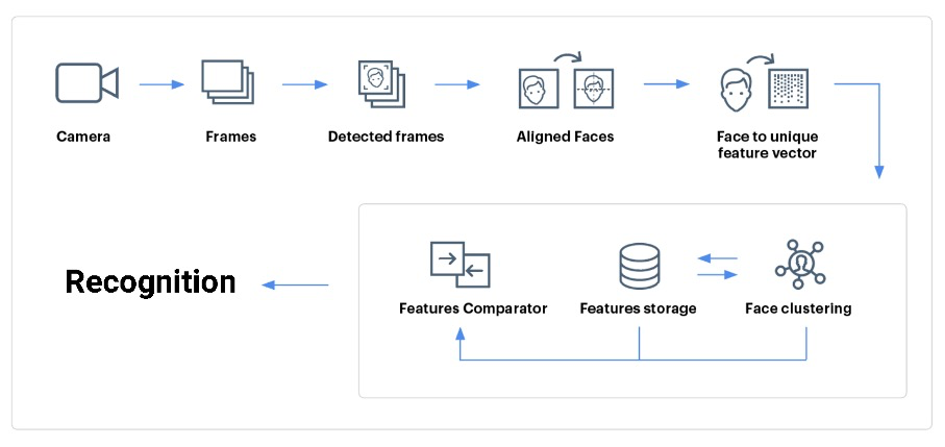
\includegraphics[width=1\textwidth]{image1-1}
\caption{نمای کلی یک سامانه تشخیص چهره}
\label{image1-1}
\end{figure}

\section{ الگوریتم‌های استخراج ویژگی و برچسب گذاری تصاویر }

\subsection{ خوشه بندی }
روش خوشه‌بندی \LTRfootnote{Clustering} بر اساس محاسبه میزان و معیار شباهت در داده‌ها، آن‌ها را در خوشه‌های مختلف قرار می‌دهد. به طور کلی دو نوع روش خوشه‌بندی وجود دارد:

\noindent
خوشه‌بندی سخت \LTRfootnote{Hard Clustering}: برچسب گذاری به صورت صفر و یک بر روی داده‌ها می‌باشد و مشخص می‌كند داده مورد نظر مربوط به خوشه می‌باشد یا خیر.

\noindent
خوشه‌بندی نرم \LTRfootnote{Soft Clustering}: به خوشه بندی فازی معروف است و عضویت یک داده به یک خوشه به کمک عددی بین صفر و یک به عنوان درجه عضویت انجام می‌شود و هر داده می‌تواند با توجه به وزن‌های اختصاص داده شده به آن، به چندین خوشه تعلق داشته باشد.

\noindent
داده‌های استفاده شده در فرایند خوشه بندی، بدون برچسب بوده و یادگیری بدون ناظر \LTRfootnote{Unsupervised Learning} در فرایند خوشه‌بندی داده‌ها استفاده می‌شود. شكل \ref{image1-2} نمونه‌ای از خوشه‌بندی سخت و یافتن شاخص برای هر خوشه را نشان می‌دهد.
\begin{figure}[!h]
\centering
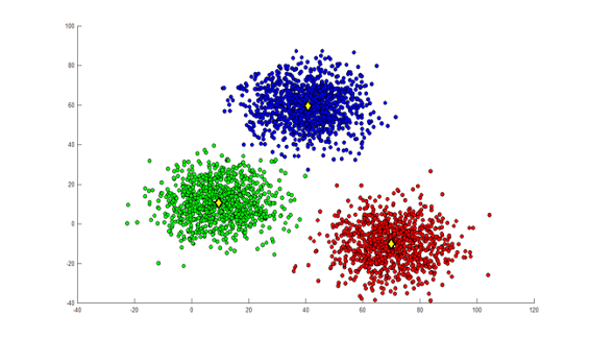
\includegraphics[scale=1]{image1-2}
\caption{ خوشه‌بندی سخت و یافتن شاخص نمونه با توزیع گوسی بر روی داده‌ها }
\label{image1-2}
\end{figure}

\subsection{طبقه‌بندی}
روش‌های طبقه‌بندی \LTRfootnote{Classification} داده‌ها از جمله روش‌های یادگیری با ناظر \LTRfootnote{Supervised Learning} هستند که با توجه به یادگیری داده‌های آموزشی به همراه برچسب آن‌ها، داده‌های آزمایشی را نیز برچسب زنی می‌کنند. در طبقه‌بندی داده‌ها می‌توان از توابع سنجش مختلفی برای سنجش میزان تعلق یک داده به هر دسته استفاده کرد. شکل \ref{image1-3} یک طبقه‌بند غیر خطی ساده را نشان می‌دهد.

\noindent
در روش‌های طبقه‌بندی که از لحاظ تعداد، بار اصلی الگوریتم‌های یادگیری ماشین را بر دوش می‌کشند، داده‌ها به دو بخش تقسیم می‌شوند. اول داده‌های ورودی (X) نامیده می‌شوند که باید بر اساس آن‌ها، فرایند پیش بینی انجام پذیرد. دوم داده‌های برچسب (Y) هستند که باید مقادیر آن‌ها پیش بینی شود. برای این منظور باید تابعی ایجاد شود که ورودی‌ها را گرفته و خروجی موردنظر را تولید کند. فرآیند یافتن این تابع، کشف رابطه‌ای بین مقادیر ورودی (X) و خروجی (Y) است که آن را فرآیند آموزش می‌نامند و تا رسیدن به دقت لازم ادامه می‌یابد. الگوریتم‌های مختلفی برای طبقه‌بندی داده‌ها وجود دارد که در این میان می‌توان به شبکه عصبی،  \lr{SVM} \LTRfootnote{Support Vector Machine} و \lr{KNN} \LTRfootnote{K Nearest Neighbor} اشاره کرد.

\begin{figure}[h]
\centering
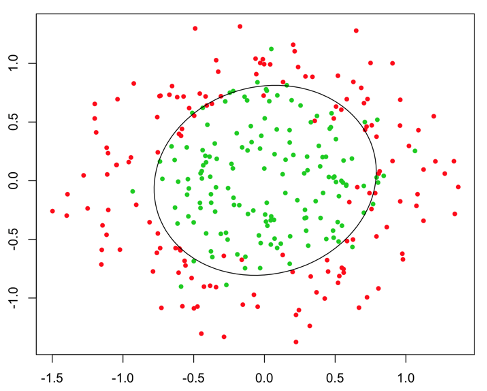
\includegraphics[scale=1]{image1-3}
\caption{ یک طبقه بند غیر خطی ساده }
\label{image1-3}
\end{figure}

\section{مسئله تشخیص بی‌درنگ چهره در محیط‌های کنترل نشده}
این پایان نامه با محوریت موضوع تشخیص بی‌درنگ چهره افراد در محیط‌های کنترل نشده با در نظر گرفتن شرایط سخت می‌باشد. هدف ما، طراحی و ساخت یک عینک هوشمند مانند شکل \ref{image1-4} برای افراد نابینا می‌باشد. هنگامی که شخص نابینا عینک را بر روی چشمانش قرار داده و در محیط‌های عمومی راه می‌رود، دوربینی که بر روی عینک نصب شده است، شروع به بررسی چهره افرادی می‌کند که در زاویه دید آن قرار دارند. در صورت یافتن یک چهره آشنا، فرد مورد نظر شناسایی شده و نام فرد برای شخص نابینا خوانده می‌شود. این مسئله شامل دو بخش اصلی یافتن چهره و شناسایی چهره می‌شود. هریک از این بخش‌ها و زیر بخش‌های آن‌ها در فصل دوم مورد بررسی قرار خواهند گرفت.

\begin{figure}[!h]
\centering
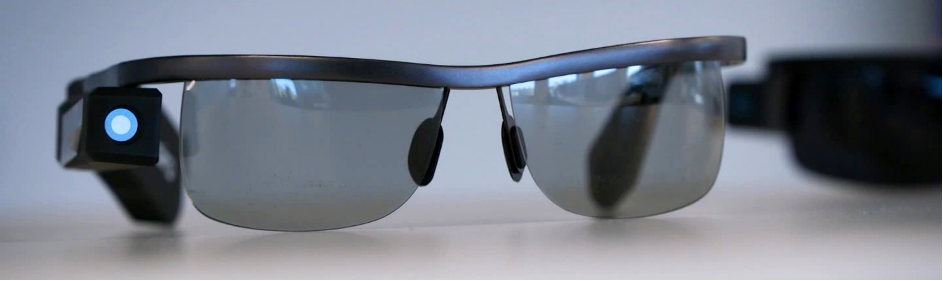
\includegraphics[width=1.0\textwidth]{image1-4}
\caption{نمونه ای از عینک دوربین دار برای افراد نابینا \cite{Glasses}}
\label{image1-4}
\end{figure}

\subsection{چالش‌های سامانه تشخیص چهره}
سامانه‌های تشخیص چهره به سطح مشخصی از بلوغ رسیده‌اند، اما توسعه آن‌ها در شرایط کنترل نشده و کاربردهای واقعی هنوز مسیر طولانی در پیش دارد. برای مثال، تشخیص چهره در ویدیو در محیطی با تغییرات شدید نورپردازی و حالت چهره، انسداد صورت، وضوح پایین تصویر و... ، و ردیابی آن در فریم‌های ویدیو با در نظر گرفتن تناظر بین فریمی و... مشکل می‌باشد. دلیل اصلی به وجود آمدن چالش‌ها این است که چهره انسان یک شی صلب نمی‌باشد و ساختار سه بعدی و پیچیده‌ای دارد و ممکن است تصویر از هر زاویه‌ای گرفته شده باشد. در ادامه مهم ترین چالش‌ها برشمرده شده است.

\noindent
نورپردازی \LTRfootnote{Lighting}: روشنایی محیط در شب و روز و یا در محیط داخلی و خارجی به شدت تغییر می‌کند. با توجه به ساختار سه بعدی چهره، یک منبع نور مستقیم می‌تواند سایه‌های قوی بر روی چهره ایجاد کند که برخی ویژگی‌های چهره را تغییر می‌دهد. همانطور که در شکل \ref{image1-5} نشان داده شده است که گاهی تفاوت‌های ظاهری ناشی از روشنایی، بیشتر از تفاوت بین چهره افراد مختلف می‌باشد.

\begin{figure}[!h]
\centering
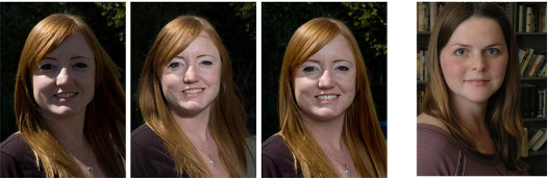
\includegraphics[scale=1]{image1-5}
\caption{مقایسه تفاوت‌های ظاهری ناشی از روشنایی و تفاوت بین چهره افراد \cite{6196234}}
\label{image1-5}
\end{figure}

\noindent
حالت \LTRfootnote{Pose}: زاویه چهره نسبت به حسگر دوربین، می‌تواند سامانه را با چالش مواجه نماید. چهره با زاویه تند و چهره‌های نیم رخ مانند شکل \ref{image1-6} باید برای الگوریتم تشخیص چهره، قابل شناسایی باشند. بنابراین ویژگی‌های استخراج شده توسط الگوریتم باید به گونه‌ای باشند که در هر زاویه‌ای امکان استخراج آن‌ها وجود داشته باشد.
\begin{figure}[!h]
\centering
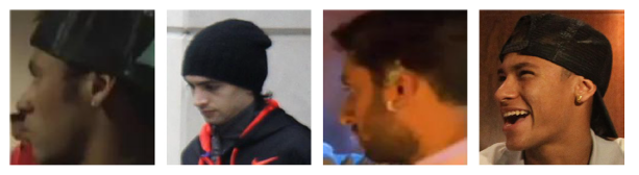
\includegraphics[scale=1]{image1-6}
\caption{زاویه شدید چهره نسبت به دوربین باعث کاهش دقت سامانه می‌شود \cite{6475017}}
\label{image1-6}
\end{figure}

\noindent
تاری خارج از تمرکز \LTRfootnote{Out Of Focus Blur}: اگر عمق میدان دوربین کم باشد و چهره‌ها با فاصله‌های مختلف از دوربین باشند، مشکل تاری خارج از تمرکز رخ خواهد داد. اگر دوربین طوری تنظیم شود که چهره نزدیک‌تر، واضح‌تر دیده شود، در مقابل باعث می‌شود که چهره دورتر، مقداری مات شود و برعکس. این مسئله می‌تواند برای سامانه تشخیص چهره دردسر ساز شود. نمونه ای از این اثر در شکل \ref{image1-7} قابل مشاهده می‌باشد.

\begin{figure}[!h]
\centering
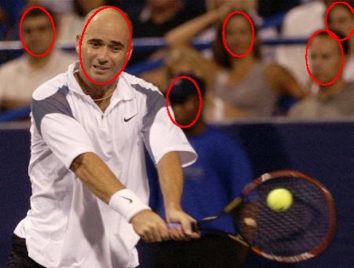
\includegraphics[scale=1]{image1-7}
\caption{تاری خارج از تمرکز به علت عمق کم میدان دوربین \cite{7477452}}
\label{image1-7}
\end{figure}

\noindent
انسداد \LTRfootnote{Occlusion}: اگر در حال تصویر برداری از یک جمع باشیم، احتمال اینکه چهره فردی توسط فرد دیگری مقداری پوشانده شود، بسیار بالاست. همچنین اگر بخشی از چهره فرد توسط موها پوشیده شده باشد، از عینک آفتابی یا ماسک استفاده کند، انسداد چهره رخ خواهد داد. نمونه ای از این اثر در شکل \ref{image1-8} قابل مشاهده می‌باشد.

\begin{figure}
	\centering
	\begin{subfigure}{.25\textwidth}
		\centering
		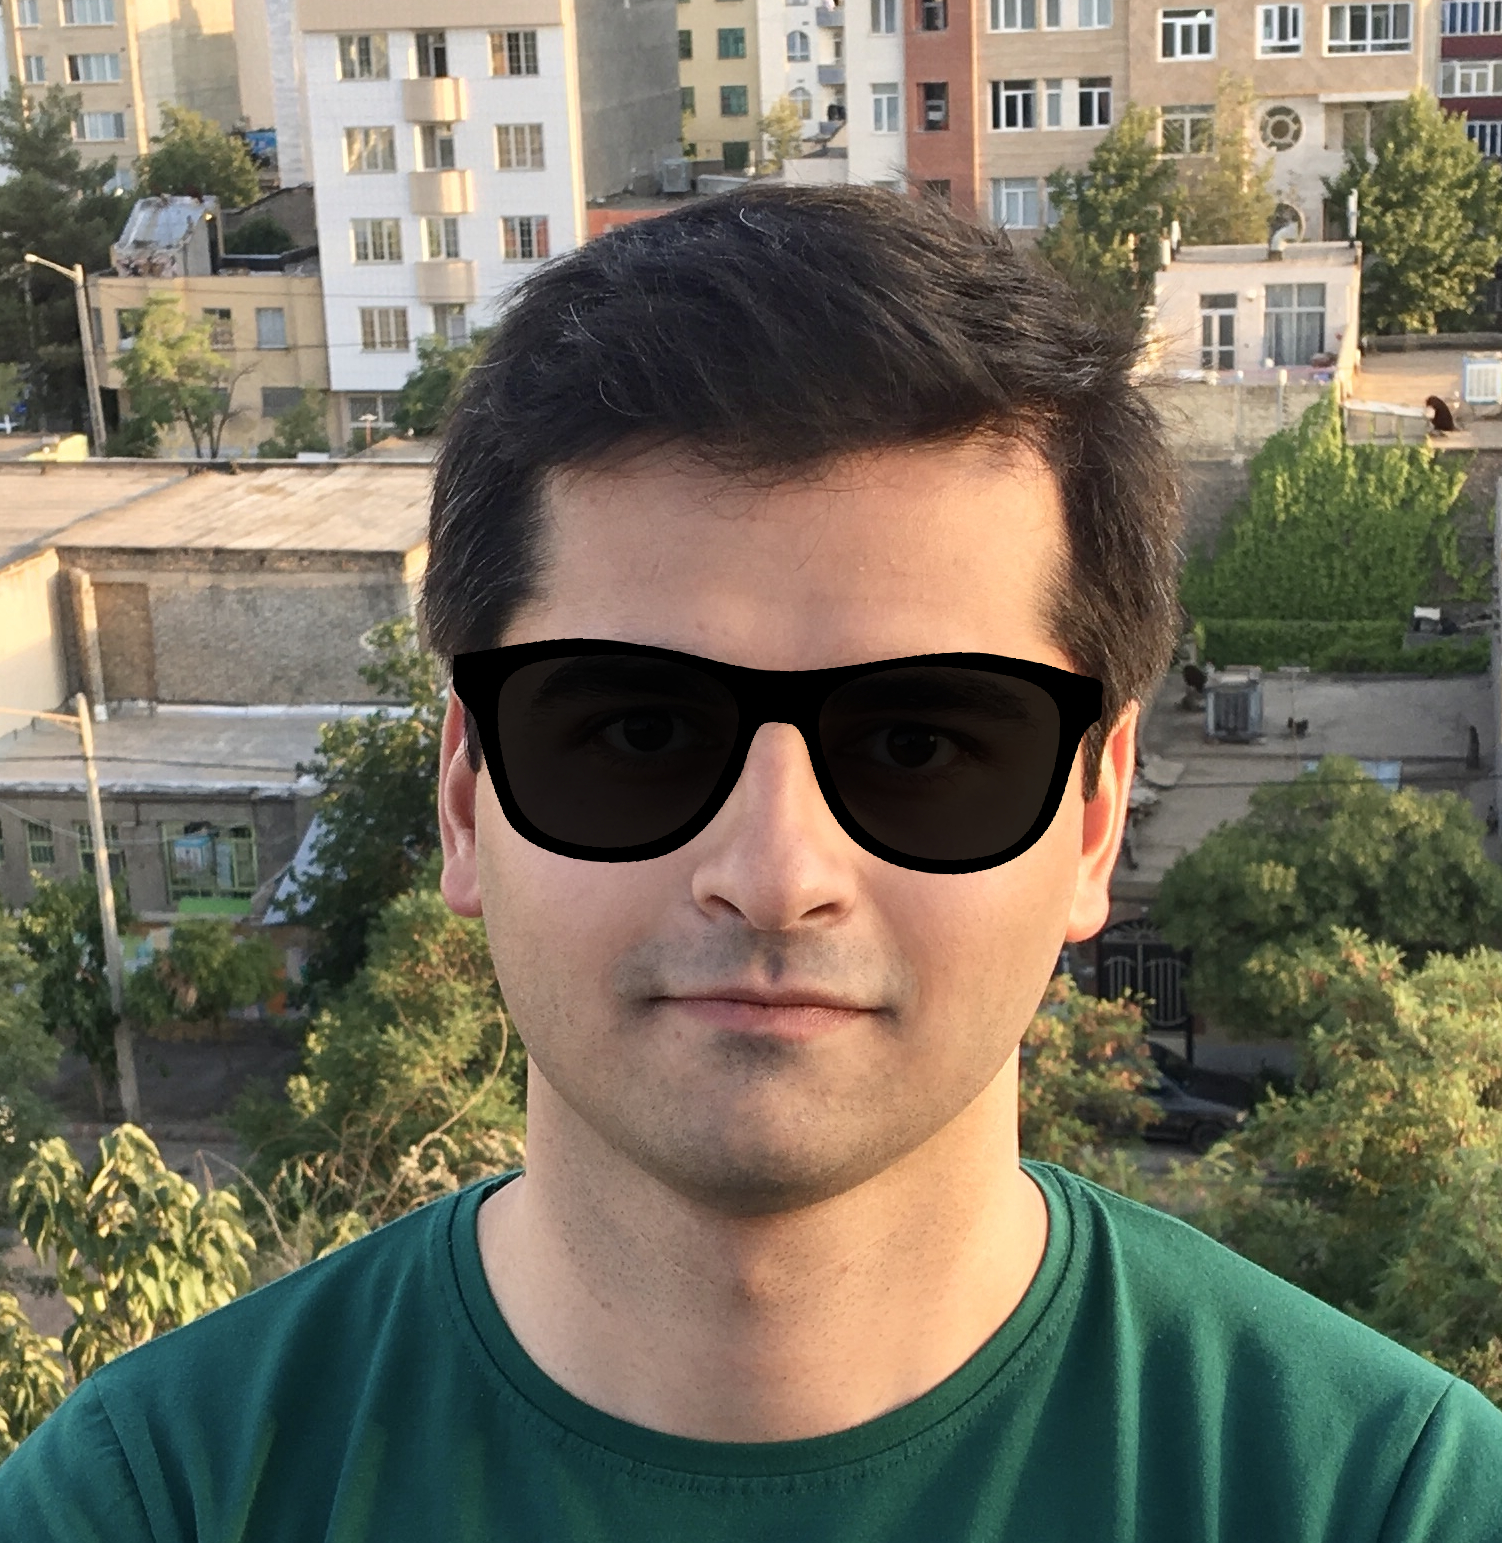
\includegraphics[width=1.0\textwidth]{image1-8-a}
		\label{image1-8-a}
	\end{subfigure}
	\begin{subfigure}{.25\textwidth}
		\centering
		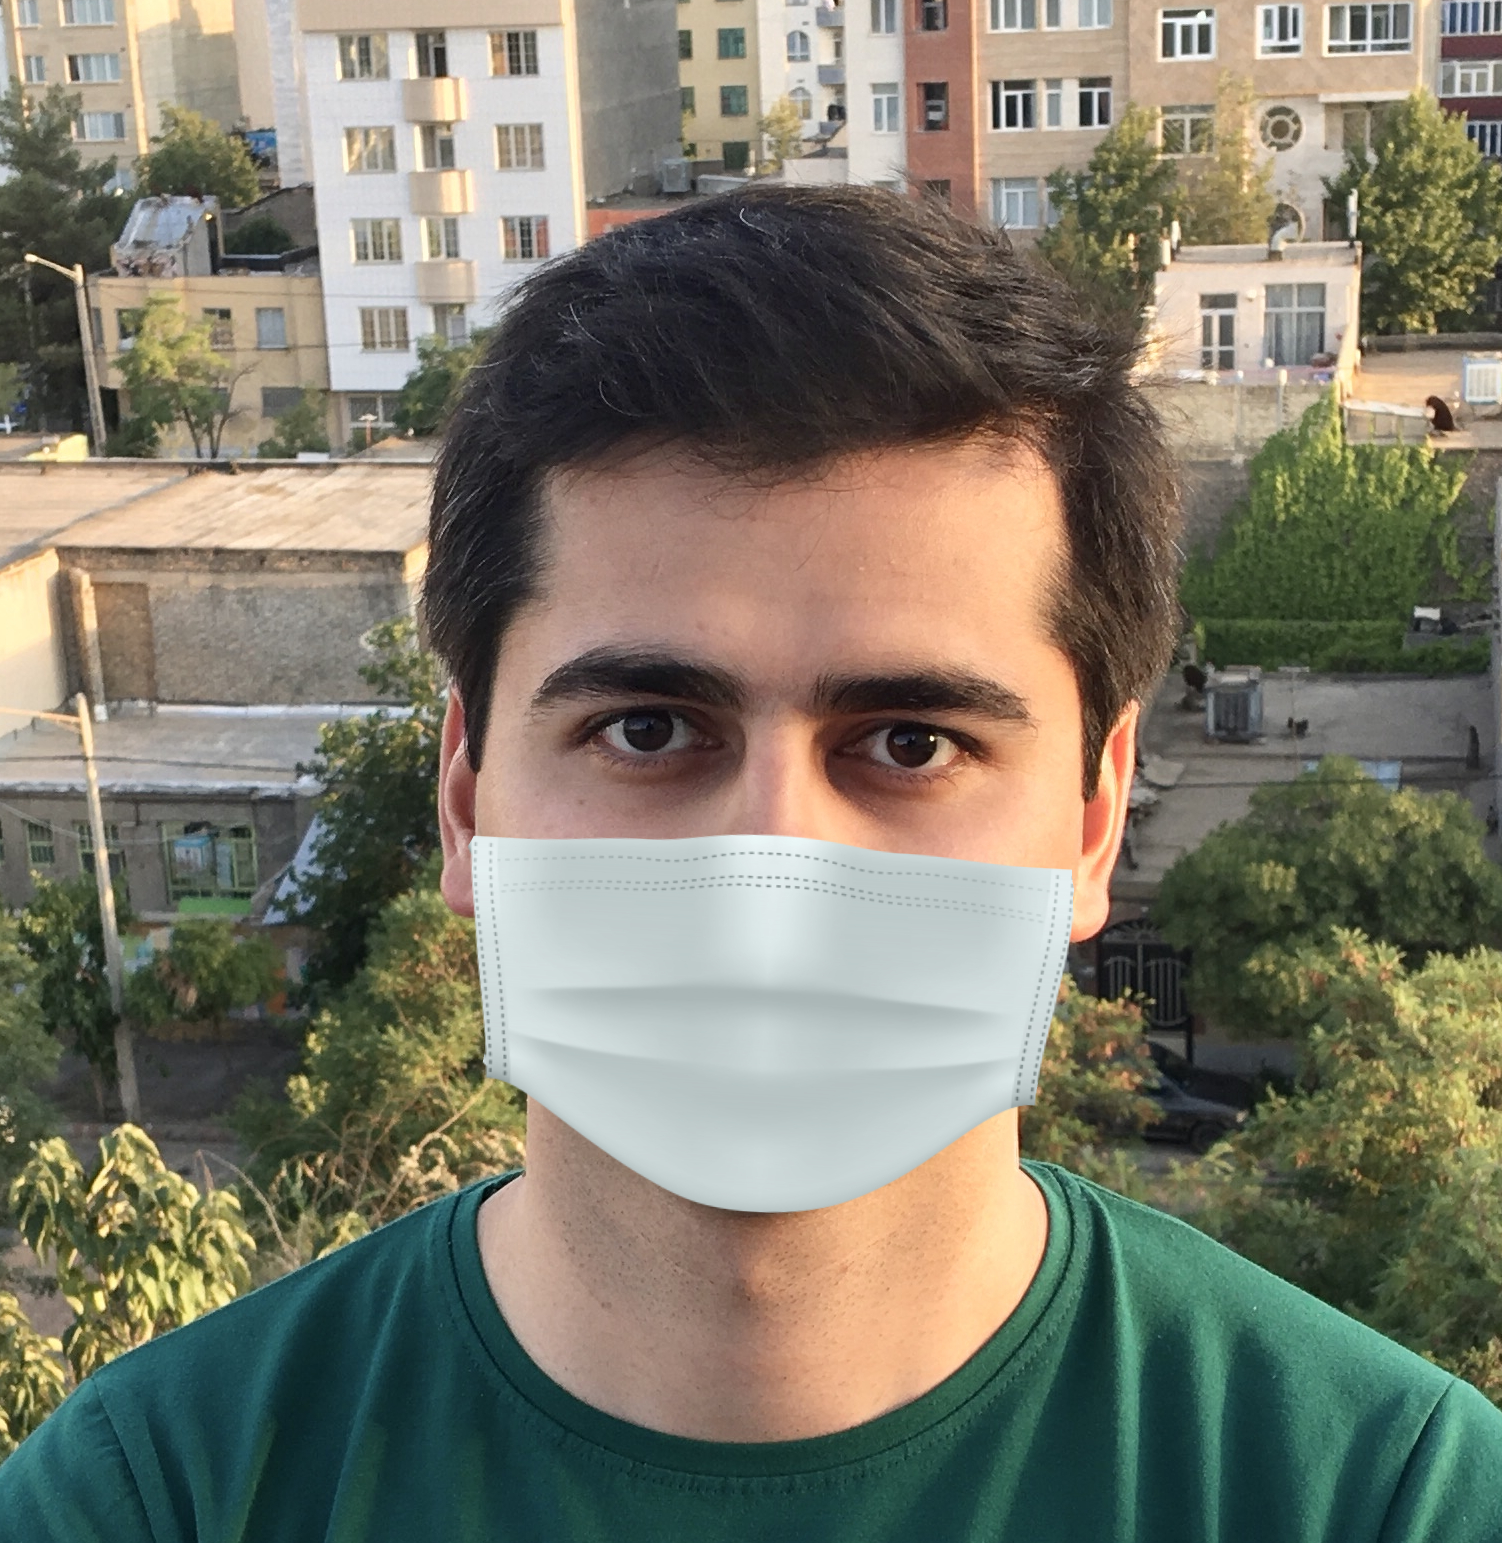
\includegraphics[width=1.0\textwidth]{image1-8-b}
		\label{image1-8-b}
	\end{subfigure}
	\caption{انسداد در اثر پوشیدن ماسک یا عینک}
	\label{image1-8}
\end{figure}

\noindent
سن \LTRfootnote{Aging}: بیشتر روش‌های مرسوم تشخیص چهره تغییرات سن را نادیده می‌گیرند. بعضی از رویکردها به طور منظم پایگاه داده تصاویر را به روز رسانی کرده و بازآموزی سامانه را انجام می‌دهند. این راه حل فقط برای سامانه‌هایی مناسب است که اغلب وظیفه احراز هویت کارمندان را انجام می‌دهد. در شرایط دیگر سن موضوع را باید جدی گرفت و تلاش کرد تا سامانه نسبت به این نوع تغییرات قوی‌تر شود.

\noindent
کمبود داده‌های آموزشی: سامانه‌های تشخیص چهره در کاربردهای واقعی دارای مشکل کمبود داده‌های آموزشی برای آموزش سامانه می‌باشند. تعداد افراد در محیط کنترل نشده زیاد می‌باشد و قادر به در اختیار داشتن حجم بالایی از داده‌های آموزشی برای هر کدام از افراد نیستیم. از طرفی کاهش تعداد داده‌های آموزشی می‌تواند دقت سامانه را به شدت کاهش دهد. 

\noindent
منابع محدود: در صورت اجرای پردازش‌های سامانه توسط تلفن همراه، باید محدودیت منابع را در نظر گرفت. تلفن همراه نسبت به رایانه، دارای قدرت پردازنده و حافظه پایین‌تر و منبع انرژی محدودتر می‌باشد که باعث می‌شود الگوریتم‌هایی با پیچیدگی محاسباتی بالا بر روی این دستگاه‌ها قابل اجرا نباشد. بنابراین الگوریتم استفاده شده باید دارای کمترین پیچیدگی زمانی و حافظه باشد.

\noindent
زمان: یکی از چالش‌های موجود، فضایی پر از چهره‌های مختلف در مکان‌های عمومی و در مقابل، نیاز به واکنش سریع توسط سامانه است. مشابه شکل \ref{image1-9} در فضاهای عمومی و معابر پیاده مردم با سرعت از کنار دوربین عبور می‌کنند و سامانه باید قابلیت تشخیص چهره آن‌ها در کسری از ثانیه را داشته باشد. اگر کاربر سامانه با افراد جدید دیدار داشته باشد، سامانه باید به سرعت یاد بگیرد که چهره افراد جدید را تشخیص دهد. 

\begin{figure}[!h]
\centering
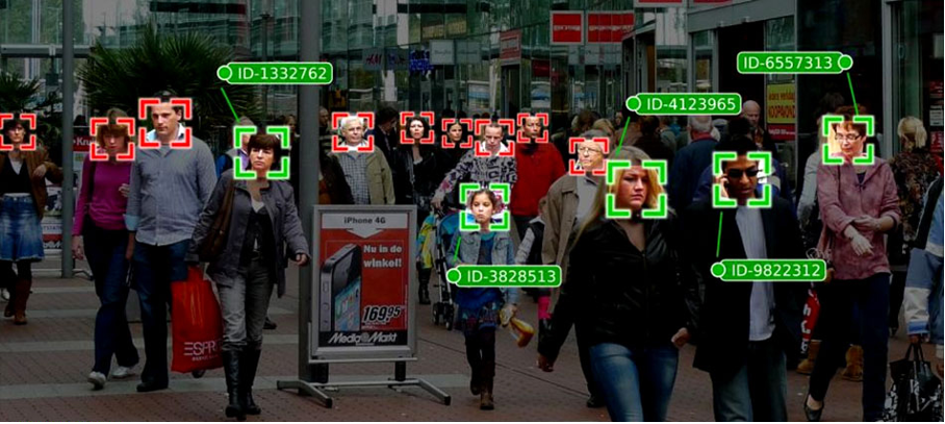
\includegraphics[width=1\textwidth]{image1-9}
\caption{نمونه ای از یک سامانه تشخیص چهره بی‌درنگ در محیط کنترل نشده \cite{CHAUDHRY2017168}}
\label{image1-9}
\end{figure}

\subsection{نوآوری‌های پایان‌نامه}
 همان‌طور که در بالا شرح داده شد، شناسایی بی‌درنگ چهره در محیط بدون محدودیت و با دقت بالا با چالش‌های بسیاری همراه است. بنابراین در این پژوهش تلاش می‌کنیم تا روشی برای تشخیص دقیق‌تر و بی‌درنگ چهره توسط شبکه عصبی عمیق در محیط بدون محدودیت پیشنهاد دهیم. در این پژوهش دو نوآوری ارائه می‌شود. اول یک معماری شبکه عصبی پیچشی به نام \lr{MobileNetV3} معرفی می‌شود که از ترکیب معماری شبکه عصبی پیچشی \lr{MobileNetV3} و یک واحد توجه به نام  \lr{MobileNetV3} می‌باشد. در ادامه تابع ضرر \lr{MobileNetV3} اصلاح شده را معرفی می‌کنیم. با استفاده از ترکیب این دو نوآوری، دقت و سرعت بالاتری نسبت به سایر روش‌های مشابه بدست می‌اوریم.  

\subsection{ساختار پایان‌نامه}
در فصل دوم به مرور رویکردهای مختلف در زمینه تشخیص چهره خواهیم پرداخت. در فصل سوم مروری بر روش‌های ارائه شده برای مواجهه با شرایط کنترل نشده خواهیم داشت. در فصل چهارم روش پیشنهادی را ارائه می‌نماییم. در فصل پنجم به ارزیابی روش پیشنهادی و مقایسه آن با سایر روش‌ها می‌پردازیم و در پایان در فصل ششم به جمع بندی و نتیجه گیری خواهیم پرداخت.